\newpage
\section{Experiment 2: Superposition of A.C and D.C. Voltages in linear and Non-linear Circuits}
\subsection{Objective}
To demonstrate the effect of applying ac and dc voltages to the same circuit simultaneously.

\subsection {Instruments}
\begin{itemize}
\item Oscilloscope
\item Low voltage DC power supply
\item 12V center tapped transformer
\item 1k$\Omega$ resistor
\item Diode
\end{itemize}

\subsection{Linear circuits - Demonstration of Superposition}
\subsubsection{Theory}
The superposition theorem states that the response in any branch of a linear circuit with multiple independent sources is the algebraic sum of the responses caused by each independent source acting alone, while all other independent sources are turned off. The superposition theorem is used to solve circuits by hand by breaking the circuit into smaller parts and analyzing each part individually. The superposition theorem is also used in circuit simulation software such as SPICE for the same purpose.
The superposition theorem is a fundamental principle in linear circuit analysis that simplifies the analysis of complex circuits. It states that in a linear circuit containing multiple independent sources, the response (voltage or current) at any element is equal to the algebraic sum of the responses caused by each independent source acting alone, with all other sources turned off.
\subsubsection{Statement of the Superposition Theorem}
Consider a linear circuit with multiple independent sources. Let \(S_1, S_2, \ldots, S_n\) be the independent sources, and \(R\) be the response (voltage or current) at a specific element in the circuit.
The total response \(R_{\text{total}}\) at the element is given by the sum of the responses caused by each source individually:
\[
R_{\text{total}} = R_{S_1} + R_{S_2} + \ldots + R_{S_n}
\]
where \(R_{S_i}\) is the response due to the \(i\)-th source acting alone, with all other sources turned off.
\subsubsection{Applicability}
The superposition theorem is applicable only to linear circuits, where the circuit elements exhibit linear relationships between voltage and current. It is particularly useful in simplifying the analysis of circuits with multiple sources, allowing engineers to focus on individual sources and their effects.
\subsubsection{Significance}
The superposition theorem provides a powerful tool for simplifying circuit analysis, especially in circuits with multiple sources. By breaking down a complex circuit into simpler sub-circuits, engineers can better understand and design electronic systems with improved accuracy.

\subsubsection{Procedure}
Construct the circuit in figure 1 \\
\begin{center}\begin{circuitikz}
    \draw 
    (0,0) node [transformer core, rotate = 90, transform shape](T){}
    % (T.inner dot B1) node[circ] {}
    % (T.inner dot B2) node[circ] {}

    (T-L1.midtap) to[R=$1K\Omega$,v=$V_0$] (0,-4) node[circ] (A){}
    (A) -- (-5,-4) to[V,v=$V_{DC}$,-|] (-5,-1.2) node[circ] (B){}
    (T-L1) -| (B)

    ;
\end{circuitikz}\end{center}
\textbf{4.1.2} Conect the primary of the transformer to the 50Hz, 240V mains. Do not turn the dc voltage on yet but connect the supply into the circuit \\

NOTE: The dc supply must be well bypassed with capacitors. However if a regulated supply is used, the bypass capacitors are not necessary. \\

\textbf{4.1.3} Measure and record the ac voltage V on the VTVM and observe the voltage V, accross the 1k$\Omega$ resistor on the scope. Sketch the waveform observed. You are advised to calibrate the vertical scale of the oscilloscope at 5 volts per division. Record and measure the peak to peak ac voltage accross R. \\

\begin{figure}[H]
    \centering
    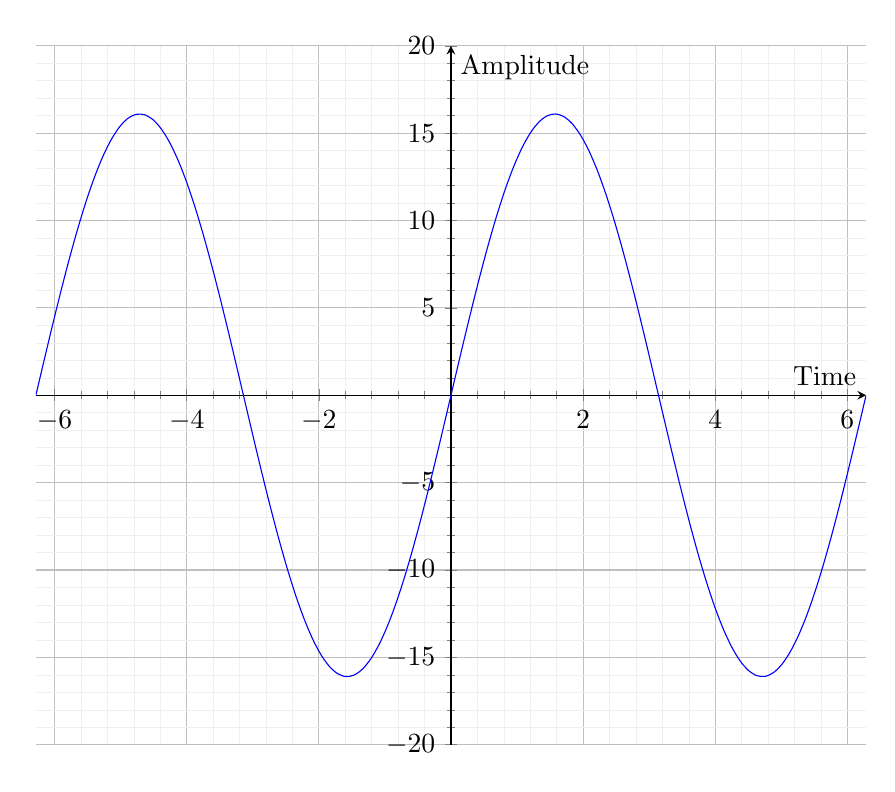
\begin{tikzpicture}
        \begin{axis}[
            xlabel={Time},
            ylabel={Amplitude},
            grid=both,
            minor grid style={very thin, lightgray!25}, 
            minor tick num = 4, 
            major grid style={thin},
            domain=-2*pi:2*pi,
            samples=100,
            xmin=-2*pi,
            xmax=2*pi,
            ymin=-20,
            ymax=20,
            width=\textwidth,
            axis lines = center,
        ]
        \addplot[blue,smooth] {16.1 * sin(deg(x))};
        \end{axis}
    \end{tikzpicture}
    \caption{Voltage accross R}
    \label{fig:ac_signal}
\end{figure}
VPP=32.2V \\


\textbf{4.1.4} Turn off the ac power supply leaving the transformer secondary connected. Apply 12V dc to terminals X-Y. Measure and record the  dc voltage accross R. \\
Vdc = 11.86V \\
\textbf{4.1.5} Now with the 12V dc still applied to the circuit, apply 240V ac to the transformer primary again. Measure the dc voltage accross R, observe the waveform of the voltage accross R on the scope sketch the waaveform observed What is the peak to peak voltage across R measured

NB: In sketching the waveform for Vo make sure to include both ac and dc components. \\

\begin{figure}[H]
    \centering
    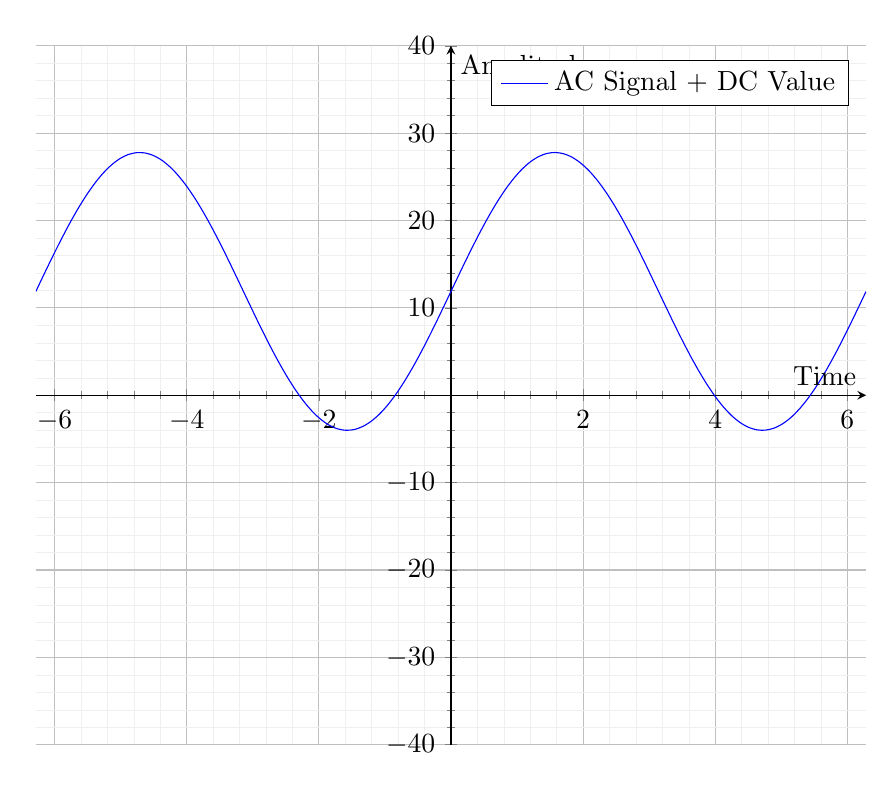
\begin{tikzpicture}
        \begin{axis}[
            xlabel={Time},
            ylabel={Amplitude},
            grid=both,
            minor grid style={very thin, lightgray!25}, 
            minor tick num = 4, 
            major grid style={thin},
            domain=-2*pi:2*pi,
            samples=100,
            xmin=-2*pi,
            xmax=2*pi,
            ymin=-40,
            ymax=40,
            width=\textwidth,
            axis lines = center,
        ]
        \addplot[blue,smooth] {15.9 * sin(deg(x)) + 11.89};  % AC signal + DC value
        \legend{AC Signal + DC Value}
        \end{axis}
    \end{tikzpicture}
    \caption{AC Signal Superposed with DC Value of 12V}
    \label{fig:ac_dc_signal}
\end{figure}
$$Vdc=11.89$$ \\
$$Vac=31.8Vpp$$ \\

\textbf{4.1.6} Now with both ac and dc applied, readjust the dc voltage to 5 volts and measure Vdc and Vac Sketch the waveform for Vo observed on the scope use the same

\begin{figure}[H]
    \centering
    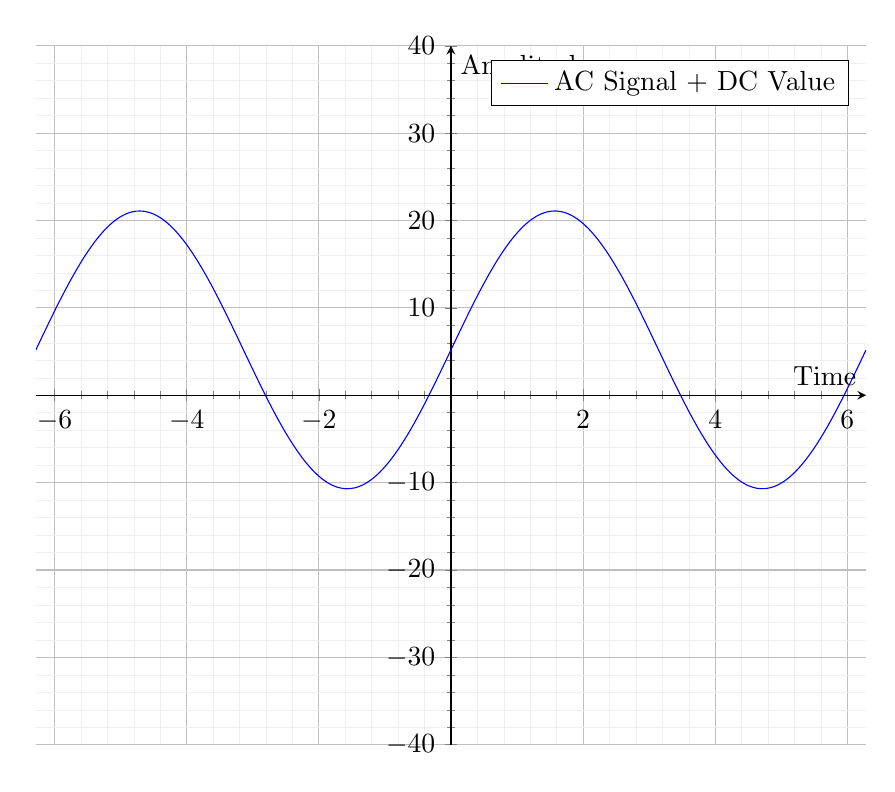
\begin{tikzpicture}
        \begin{axis}[
            xlabel={Time},
            ylabel={Amplitude},
            grid=both,
            minor grid style={very thin, lightgray!25}, 
            minor tick num = 4, 
            major grid style={thin},
            domain=-2*pi:2*pi,
            samples=100,
            xmin=-2*pi,
            xmax=2*pi,
            ymin=-40,
            ymax=40,
            width=\textwidth,
            axis lines = center,
        ]
        \addplot[blue,smooth] {15.9 * sin(deg(x)) + 5.20};  % AC signal + DC value
        \legend{AC Signal + DC Value}
        \end{axis}
    \end{tikzpicture}
    \caption{AC Signal Superposed with DC Value of 5V}
\end{figure}
$$Vdc=5.20$$ \\
$$Vac=31.8Vpp$$ \\
\subsubsection{Discussion}
\subsection{Analysis Questions}

\subsubsection{1. State whether the DC level has any significant effect on the part of the value of the AC voltage.}

The DC level does not have a significant effect on the amplitude of the AC voltage. According to the principle of superposition, in a linear circuit, the DC and AC components can be analyzed separately. The DC level sets the bias point, while the AC signal fluctuates around this bias. The amplitude of the AC signal is determined by the AC source, and the DC level does not impact it.

\subsubsection{2. What happens to the DC level when the AC voltage is turned off?}

When the AC voltage is turned off, the DC level remains unaffected. The DC component is a steady-state value that represents the average voltage or bias in the circuit. Turning off the AC source only removes the fluctuating AC signal, leaving the DC level unchanged.

\subsubsection{3. What basic property of linear circuits is demonstrated by this experiment?}

This experiment demonstrates the linearity of the circuit. Linearity implies that the circuit follows the principle of superposition, allowing separate analysis of the DC and AC components. The behavior of the circuit is consistent and predictable when subjected to varying input signals.

\subsubsection{4. State this principle and briefly explain what it means.}

The principle of superposition states that in a linear circuit, the response (voltage or current) at any point is the algebraic sum of the individual responses caused by each independent source acting alone, with all other sources turned off. This means that the effects of individual sources can be analyzed independently and then combined to determine the overall response of the circuit.


\subsection{Non-linear circuits}

\subsubsection{Theory}
The superposition theorem is a fundamental concept in linear circuit analysis, allowing for the simplification of complex circuits with multiple independent sources. However, it is crucial to understand that superposition is valid only for linear circuits, where the relationship between voltage and current is linear. In nonlinear circuits, components exhibit non-linear behavior, and applying superposition directly may lead to inaccuracies.
\subsubsection{Nonlinear Components}
Nonlinear components, such as diodes and transistors, introduce non-linear relationships between voltage and current. Unlike resistors, these components do not follow Ohm's law, making the application of superposition challenging.
To investigate the limitations of the superposition theorem in nonlinear circuits, consider a circuit with a nonlinear element, such as a diode. Design the circuit to include multiple independent sources and resistors along with the nonlinear component.
\subsubsection{Significance}
This experiment aims to highlight the limitations of applying superposition to nonlinear circuits. By comparing the superposition-based predictions with actual measurements, you can illustrate the impact of non-linear elements on the accuracy of the superposition theorem.


\subsubsection{Procedure}
\textbf{5.1.1} Construct the circuit in figure 2. \\

\begin{center}\begin{circuitikz}
    \draw 
    (0,0) node [transformer core, rotate = 90, transform shape](T){}
    (-5,-6) node[circ] (B){}
    % (T.inner dot B1) node[circ] {}
    % (T.inner dot B2) node[circ] {}
    (T-L1) -| (-5,-1)node[circ](A){} 
    (B) to[V,v=$V_{DC}$,-|] (A) 
    (B) -- (3,-6) node[circ](N){N} 
    (N) to[R=$1K\Omega$,v=$V_0$] (3,-3) node[circ] (M){M}
    (M) to[Do] (3,-1) node[circ] (L){L} -| (T-L1.midtap)
    ;
\end{circuitikz}\end{center}
\textbf{5.1.2} Connect the primary of the transformer to the 50Hz, 240V mains. Do not turn the dc voltage on yet but connect the supply into the circuit. \\
\textbf{5.1.3} With the vertical input of thr oscilloscope calibvrated to 5V per division, connect thew scope common to M and the probe to L. Sketch the wave form observed  \\
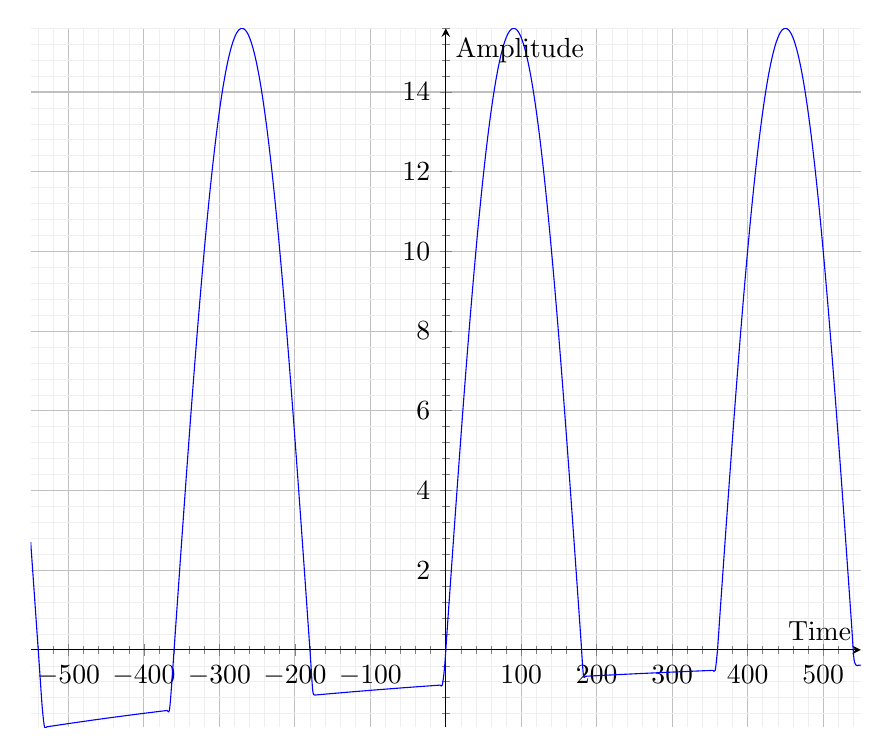
\begin{tikzpicture}
    \begin{axis}[
        xlabel={Time},
        ylabel={Amplitude},
        grid=both,
        minor grid style={very thin, lightgray!25}, 
        minor tick num = 4, 
        major grid style={thin},
        % domain=-2*pi:2*pi,
        samples=100,
        % xmin=-2*pi,
        % xmax=2*pi,
        % ymin=-40,
        % ymax=40,
        width=\textwidth,
        axis lines = center,
        domain=-550:550,
        samples=360,
        axis lines=center,
    ]
    \addplot[blue, smooth] {max(15.6*sin(x), -exp(-(0.0015*mod(x+90, 720))))};
    \end{axis}
    \end{tikzpicture}
   
$$Vac= 15.6Vpp$$ \\
\textbf{5.1.4} with the scope common still at N, connect the probe to M. Sketch the waveform observed \\
\begin{figure}[H]
    \centering
    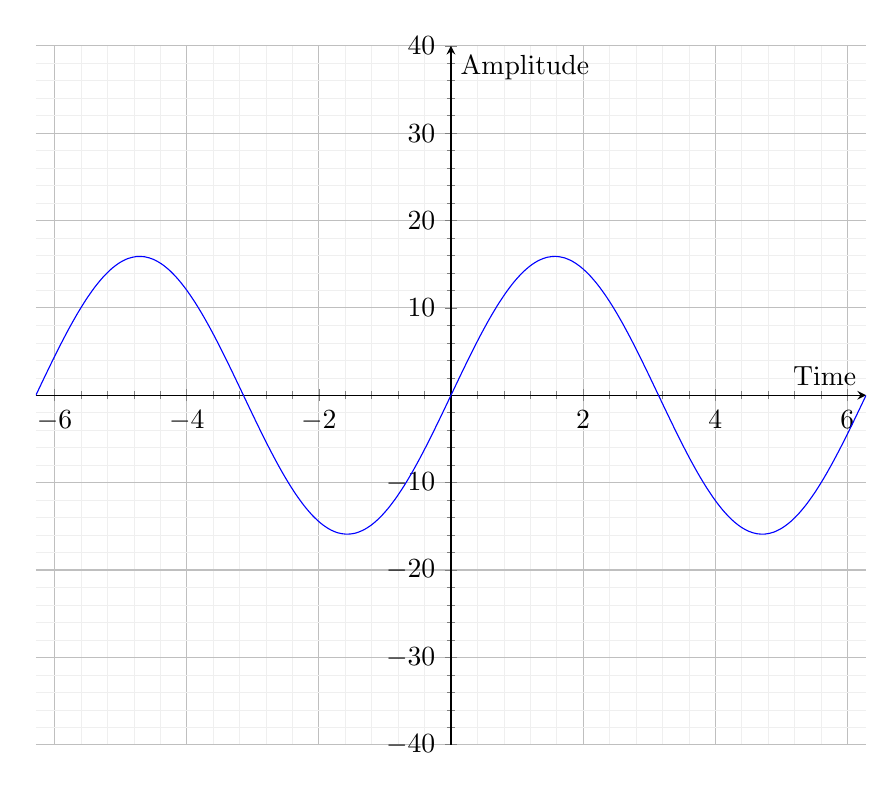
\begin{tikzpicture}
        \begin{axis}[
            xlabel={Time},
            ylabel={Amplitude},
            grid=both,
            minor grid style={very thin, lightgray!25}, 
            minor tick num = 4, 
            major grid style={thin},
            domain=-2*pi:2*pi,
            samples=100,
            xmin=-2*pi,
            xmax=2*pi,
            ymin=-40,
            ymax=40,
            width=\textwidth,
            axis lines = center,
        ]
        \addplot[blue,smooth] {15.9 * sin(deg(x))};  % AC signal + DC value
        % \legend{AC Signal + DC Value}
        \end{axis}
    \end{tikzpicture}
    \caption{AC Signal Superposed with DC Value of 5V}
\end{figure}
$$Vdc=5.20$$ \\
$$Vac=31.8Vpp$$ \\
\textbf{5.1.5} Next move the scope common to M and connect the probe to L. Sketch the waveform observed \\
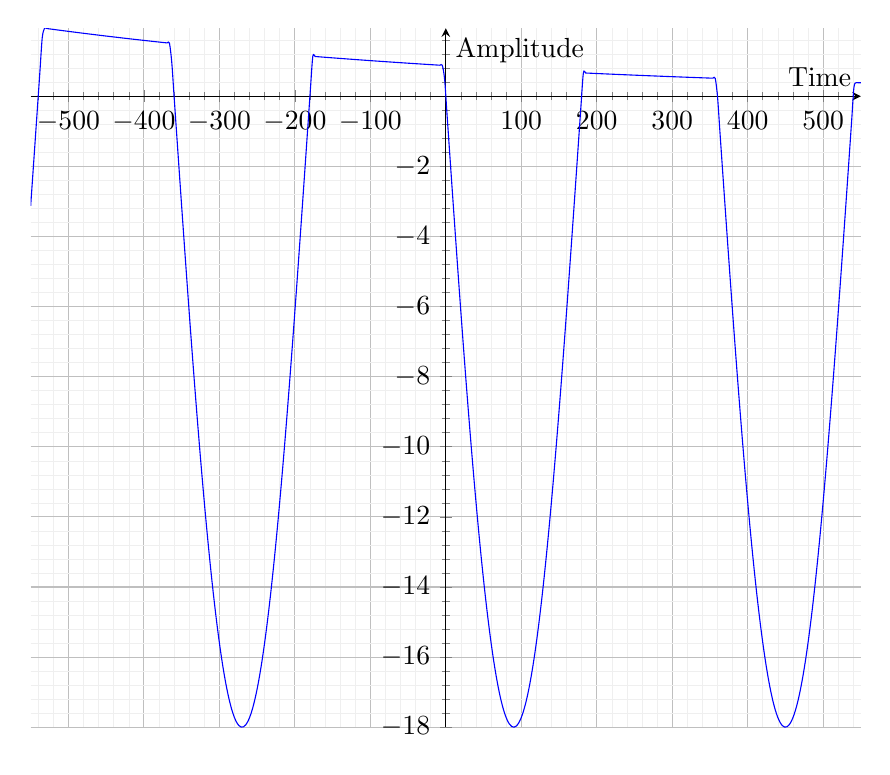
\begin{tikzpicture}
    \begin{axis}[
        xlabel={Time},
        ylabel={Amplitude},
        grid=both,
        minor grid style={very thin, lightgray!25}, 
        minor tick num = 4, 
        major grid style={thin},
        % domain=-2*pi:2*pi,
        samples=100,
        % xmin=-2*pi,
        % xmax=2*pi,
        % ymin=-40,
        % ymax=40,
        width=\textwidth,
        axis lines = center,
        domain=-550:550,
        samples=360,
        axis lines=center,
    ]
    \addplot[blue, smooth] {-max(18*sin(x), -exp(-(0.0015*mod(x+90, 720))))};
    \end{axis}
    \end{tikzpicture}
   
$$Vac= 18.0Vpp$$ \\
\textbf{5.1.6} Now with the ac still applied to the circuit, apply 5V dc  accross the terminals L-N.

\textbf{5.1.7} With the scope common still at N, connect the probe to L. Sketch the waveform observed. \\
\begin{figure}[H]
    \centering
    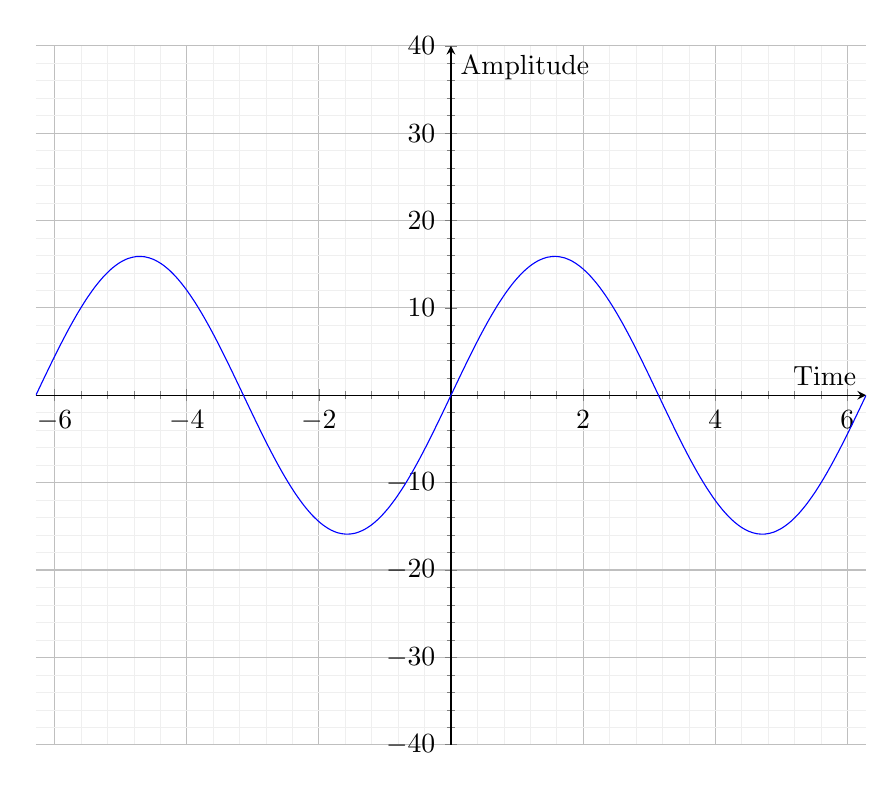
\begin{tikzpicture}
        \begin{axis}[
            xlabel={Time},
            ylabel={Amplitude},
            grid=both,
            minor grid style={very thin, lightgray!25}, 
            minor tick num = 4, 
            major grid style={thin},
            domain=-2*pi:2*pi,
            samples=100,
            xmin=-2*pi,
            xmax=2*pi,
            ymin=-40,
            ymax=40,
            width=\textwidth,
            axis lines = center,
        ]
        \addplot[blue,smooth] {15.9 * sin(deg(x))};  % AC signal + DC value
        % \legend{AC Signal + DC Value}
        \end{axis}
    \end{tikzpicture}
    \caption{AC Signal}
\end{figure}
$$Vdc=5.20$$ \\
$$Vac=31.8Vpp$$ \\
\textbf{5.1.8} Next move the scope common to M and connect the probe to L. Sketch the waveform observed. \\
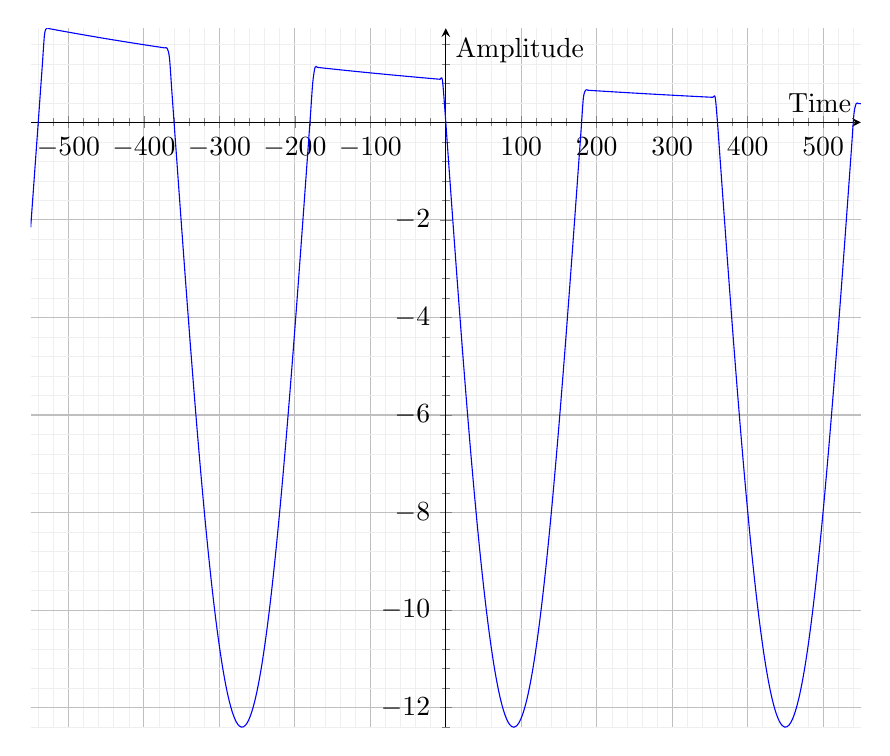
\begin{tikzpicture}
    \begin{axis}[
        xlabel={Time},
        ylabel={Amplitude},
        grid=both,
        minor grid style={very thin, lightgray!25}, 
        minor tick num = 4, 
        major grid style={thin},
        % domain=-2*pi:2*pi,
        samples=100,
        % xmin=-2*pi,
        % xmax=2*pi,
        % ymin=-40,
        % ymax=40,
        width=\textwidth,
        axis lines = center,
        domain=-550:550,
        samples=360,
        axis lines=center,
    ]
    \addplot[blue, smooth] {-max(12.4*sin(x), -exp(-(0.0015*mod(x+90, 720))))};
    \end{axis}
    \end{tikzpicture}
   
$$Vac= 12.4Vpp$$ \\


\subsection{Conclusion}

While the superposition theorem is a powerful tool in linear circuit analysis, its direct application to nonlinear circuits can lead to errors. Understanding these limitations is crucial for accurate analysis and design of circuits containing nonlinear components.
